%!TEX root = ../main.tex

\chapter[Character Bias in the Cultural Success of Fairy Tales]{Devils, fairies and dragons: Character bias in the cultural success of fairy tales}\label{ch:animacy}

\chapterprecishere{
``Suppose we get the Professor to tell us a story.''\\
Bruno adopted the idea with enthusiasm. Please do. he cried eagerly. ``Sumfin about tigers--and bumble-bees--and robin-redbreasts, oo knows!''\\
``Why should you always have live things in stories?'' said the Professor. ``Why don’t you have events, or circumstances?''\\
``Oh, please invent a story like that!'' cried Bruno.\\
The Professor began fluently enough. ``Once a coincidence was taking a walk with a little accident, and they met an explanation--a very old explanation--so old that it was quite doubled up, and looked more like a conundrum--'' he broke off suddenly.\\
``Please go on!'' both children exclaimed.\\
The Professor made a candid confession. ``It’s a very difficult sort to invent, I find. Suppose Bruno tells one first.''\\
Bruno was only too happy to adopt the suggestion.\\
``Once there were a Pig, and a Accordion, and two jars of Orange-marmalade''
}{Lewis Carroll}{Sylvie and Bruno Concluded}

\section{Introduction}\label{sec:cultural-success-intro}

With his 2006 monograph \emph{Why fairy tales stick}, Jack Zipes addresses perhaps the most central question in fairy tale transmission research: why does it seem that fairy tales consistently succeed to prevail in culture?\autocite{zipes:2006} Among the most popular stories in present-day Western Culture are fairy tales like ``Cinderella'', ``Snow White'' or ``Red Riding Hood'' -- all of which are not present-day creations but find their roots in centuries-old tales. In recent research, it has even been suggested that fairy tales might even be much older than their first literary record, evidence suggesting that tales such as ``The Smith and the Devil'' can be traced back to the Bronze age.\autocite{daSilva:2016} Observations such as these have led many to believe that there is something about fairy tales that makes them stick.

But not \emph{all} fairy tales stick. While we have all undoubtedly heard of ``Cinderella'' or ``Red Riding Hood'', it seems that we are much less familiar with the story of ``The Poor Boy in the Grave'' or ``The Jew in the Brambles'' -- if we are aware of these stories at all. In the 1857 edition of the fairy tale collection \emph{Kinder- und Hausmärchen}, the Brothers Grimm collected and published as much as 210 stories; yet, only a handful of them is included in the present-day canon\autocite{zipes:2006,joosen:2014}. The question, then, should not be `why fairy tales stick', but rather `\emph{which} fairy tales stick', and why it is precisely those that prevail.

In the existing literature, some suggestions have been made regarding the appeal of `stories that stick'. There are a number of experimental studies of story transmission in a laboratory context using a transmission chain method \autocite{bartlett,Lyons:2006,mesoudiwhiten:2010,breithaupt:2015}. In a laboratory setting, stories are passed down either orally or in writing from one participant generation to the next under controlled conditions. Results from such experimental simulation studies suggest that the progressive alterations of stories are primarily controlled by social and cognitive selection pressures\autocite[See e.g.][]{owens:1979,diehl:2006,mesoudiwhiten:2008,eriksson:2012}. It has been shown, for example, that story elements are preferred to be selected for transmission when they convey minimally counterintuitive concepts, rather than intuitive or counterintuitive concepts\autocite{barrett:2004,Norenzayan:2006,Upal:2011}. A concept is considered to be minimally counterintuitive when most of its characteristics are in accordance with the ontological assumptions of the concept, yet a few characteristics are not consistent with these assumptions\autocite{Norenzayan:2004}. An example of a minimally counterintuitive concept is that of a ghost; a ghost shares many characteristics with other intentional agents (e.g.\ consciousness, feelings, beliefs), yet a few of its characteristics, such as its being invisible and ability to move through walls, go against the ontological assumptions about intentional agents. Experimental evidence has shown that such minimally counterintuitive concepts are more memorable and are more accurately transmitted than intuitive or counterintuitive concepts. Furthermore, in a corpus study, \citeauthor{Norenzayan:2006} have shown that narratives consisting of a few (typically in the range of 2 to 3) minimally counterintuitive concepts have a transmission advantage over other stories.\autocite{Norenzayan:2006} Other examples of selectional preferences include salient story elements, or rather, story elements evoking heavy emotional reactions such as disgust\autocite{eriksson:2014}, and a disposition for social information\autocite{reysen:2011,Stubbersfield:2014}. For instance, stories containing a high degree of `gossip-like' information (such as romantic intrigues between students and professors) are more likely to be accurately transmitted, and therefore have a higher probability of persisting in their original form\autocite{mesoudi:2006}.

However, while such experimental studies in laboratory contexts implicitly affect our understanding of story transmission in the real world, their results cannot be unequivocally taken to apply to real-world story transmission and selection phenomena. Observations regarding real-world data, specifically concerning fairy tale transmission and the canonization of the Brothers Grimm, have been made by \citeauthor{joosen:2014}, who suggests that successful fairy tales dominantly revolve around female characters. A study by \citeauthor{koman:2008} remarkably points in a similar direction: of the ten most popular fairy tales in the Dutch language area, seven are centered around female characters and the top four contain a single female protagonist.\autocite[I.e.\ ``Snow White'', ``Cinderella'', ``Sleeping Beauty'', and ``Red Riding Hood'', cf.][]{koman:2008} Yet, female protagonists are not the only recurring character type in the most popular fairy tales; the top three stories all contain a cruel witch or stepmother as an antagonist character and a prince who the protagonists end up marrying. As such, it appears that female protagonists are but one of many possible appealing traits of a story. 

Interestingly, neither the experimental research, nor story transmission research in literary and folkloristic studies seems to devote attention to what makes certain stories \emph{unsuccessful}. In both research areas, the main object of interest are the stories that remain after a repeated `filter-and-selection' process in cultural transmission, and the questions asked centered on the traits that distinctively define the persisting stories. However, the distinctive traits of unpopular stories are largely ignored. Of course, by determining popular traits, scholars imply that it is the \emph{lack} of popular characters that makes particular stories less popular and causes them to disappear from cultural memory, but the idea that there might be such a thing as `impopularizing' traits or characters, making a story less interesting or appealing for further transmission, has thus far been consistently overlooked.

It is these questions and remaining hiatuses in the understanding of what determines selection in fairy tale transmission that I will address in the present chapter. I will systematically examine fairy tales from the Brothers Grimm collection with varying degrees of successfulness. By developing a folktale character typology, and subsequently mapping the characters from the Grimm's fairy tales to this typology, I provide empirical evidence for several character types that discriminate between popular and impopular tales. The results indicate that popular tales revolve around what can be considered `minimally counterintuitive characters', such as `ghosts', `dwarfs', `giants' and `witches'. In addition, we also find that characters in the sphere of close social family relations, such as `siblings' and `parents', are commonly found in successful stories. Unsuccessful stories, by contrast, appear to be centered around characters from the religious sphere, comprising `priests' and `popes' as well as `Jesus' and `God'. Besides biblical and cleric characters, unpopular stories also tend to stage generic or collective characters, which do not represent a single, definite (and, hence, more personal) entity, but a more indeterminate group of a particular kind or type of people, such as `men', `thieves' and `people'. These findings serve to aid our understanding of how the funnel-like selection process observed in the dissemination of the 210 stories in \emph{Kinder- und Hausmärchen} has proceeded, which, in its turn furthers the understanding of the more general question of how to explain prevalent culture, in which some cultural artifacts are more likely to survive than others.

Besides its general theoretical relevance, addressing the question of which characters correlate with popular and impopular stories in such a large-scale collection as \emph{Kinder- un Hausmärchen} poses an important methodological challenge. The present chapter presents a computational system that automatically extracts the character cast of stories using a mechanism that detects animate behavior of entities in texts. This model, which serves as the methodological base for the further research questions on story transmission addressed here, will be set out and described in detail in the next section (Section \ref{sec:animacy}). Section \ref{sec:grimmpopularity}, then, will return to the central question of this chapter. Here, the animacy detection model will be applied to the Grimm's fairy tale collection, yielding a list of all characters in all stories. Based on these lists, we can determine which character types distinctively occur in popular and impopular stories. Finally, the interpretation and theoretical implications of these results will be presented in Section \ref{sec:animacydiscussion}.


\section{Animacy Detection in Stories}\label{sec:animacy}

For almost all species in the world, the capacity to distinguish animate objects from inanimate objects is essential to their survival. Those objects could be prey, for example, or predators or mates. The fundamental nature that the distinction between animate and inanimate has for humans is reflected in the fact that this division is acquired very early in life: children of less than six months old are well able to distinguish the two categories from one another\autocite{opfer:2002}. Moreover, recent brain research shows that the distinction appears in the organization of the brain\autocite{gao:2012}. For some researchers, this provides evidence for the idea that the division between animate and inanimate is an innate part of how we see the world.

Although animacy may be a scalar rather than a strictly categorical distinction\autocites[See e.g.\ the animacy hierarchy in][]{comrie:1989}[and research such as][]{rosenbach:2008}, the distinction between animate and inanimate is traditionally taken as binary with regard to lexical items: something is either animate (e.g.\ a human) or not (e.g.\ a chair). This standpoint has been challenged, however, by researchers from different fields. Firstly, it has long been established in linguistic typology that not all languages award animacy to the same entities in different grammatical categories. As \citeauthor{comrie:1989} notes, for example, English, and many other languages, distinguishes between human and not-human in the choice of pronouns, whereas Russian distinguishes between animate (entailing humans and animals) versus non-animate (entailing everything else) in its interrogative pronouns\autocite{comrie:1989}. Another example indicating different subdivisions of animacy in languages is found in Persian. In English, \emph{tree} and \emph{flower} are both inanimate words, but in Persian the word for \emph{tree} is grammatically classified as animate, whereas the word for \emph{flower} is classified as being \emph{inanimate} along with words such as \emph{house} and \emph{chair}.\autocite[211]{wiese:2003} Secondly, philosophers such as Daniel Dennett support the view that animacy and aliveness are to be treated as epistemological stances rather than fixed states in the world: not ineffable qualia but behavioral capacity defines our stance towards objects\autocite{dennett:1996}. In other words, depending on whether people \textit{think} that an object is animate, they utilize different cognitive strategies to explain and predict the actions of those objects. Finally, evidence from psycholinguistic research has accumulated to support this view of animacy as a cognitive viewpoint rather than an extra-perceptive absolute. \citeauthor{nieuwland:2005}, for example, show that college student test subjects readily accept animate behavior from inanimate objects within the proper contexts\autocite{nieuwland:2005}, and \citeauthor{vogels:2013} moreover emphasize the relation between animacy and motion, showing that factors such as self-propelment play a crucial role in recognizing and/or awarding animacy to certain objects\autocite{vogels:2013}. This is exemplified in the opening of this well-known story:\footnote{Taken from: \url{http://www.verhalenbank.nl/items/show/9636}.}
\begin{quote} 
    A farmer bought a pancake on the market. Once he got home, the farmer was hungry and began to bake the pancake. The farmer tried one of his skillful flipping techniques, but he failed and the pancake fell on the ground. Coincidentally, the door of the kitchen was open and the pancake rolled out to the field, as hard as he could\ldots
\end{quote}
Although initially, based on their knowledge of the world, readers will regard the pancake as inanimate, the self-propelled motion verb `rolled' initiates our shift towards an animate interpretation of the pancake. As readers (or listeners) of a story, we choose to view participating objects at varying levels of abstraction in order to predict their behavior. \citeauthor{dennett:1996} defines three levels of abstraction: (i) the `physical stance', (ii) the `design stance' and (iii) the `intentional stance'\autocite{dennett:1996}. The physical stance deals with predictions about objects given their physical properties. The design stance deals with concepts such as purpose, function or design. The intentional stance is concerned with belief, thinking and intentions. These are all cognitive strategies we use to predict and explain the actions of objects in our environment. Interestingly, in the process of reading the opening of the story about the fleeing pancake, readers and listeners experience the transition from one strategy to the next quite clearly. Initially, the pancake is interpreted from a physical stance, or perhaps the more abstract design stance in terms of the purpose (i.e.\ to stave off hunger). It is only at the last adverbial phrase `as hard as he could' that we start to wonder whether we should adopt to the yet more abstract intentional stance and consider the pancake to be a rational agent.

Given the fundamental nature of the distinction between animate and inanimate, it is perhaps not too surprising that it has proven to be invaluable in a variety of Natural Language Processing tasks dealing with e.g.\ anaphora resolution and dependency parsing\autocite{orasan:2007,lee:2013,ovr:niv:2007}. Existing methods for the automatic labeling of text for animacy are usually rule-based, machine-learning-based, or a hybrid of these methods. Common to most approaches is the fact that they make use of semantic lexicons with information about animacy, as well as syntactic cues in a text. Both feature types are relatively costly to obtain as they require large vocabularies or syntactic parsing systems, which, with the exception of a few languages, are not readily available.

In this chapter, I present a new linguistically uninformed model to automatically label texts for animacy. It is shown that we can do away with features that require syntactic parsing or semantic lexicons while still yielding competitive performance. The focus is on labeling animacy in stories, because stories pose some interesting problems to automatic systems of animacy recognition. As the example of the fleeing pancake already illustrated, in stories any entity may at some point exhibit animate behavior, even when they are inanimate in the `real' world. Another example is the \textit{Sorcerer's Apprentice} sequence in Walt Disney's famous \textit{Fantasia}, in which brooms display the ability to collect buckets of water. Such examples, in which entities such as pancakes and brooms act as animate beings, make a clear case for developing dynamic, data driven systems that do not rely too much on static and fixed world knowledge, but rather on immediate context.

The remainder of this section is structured as follows. I will start with a short overview of existing techniques for automatically labeling animacy in texts, including the definitions of animacy used in these papers (Section \ref{sec:animacy-previous-work}). After a description of the corpus used in this study and how the annotations of the corpus have been established (Section \ref{sec:animacy-data}), I will give an account of the computational models in Section \ref{sec:animacy-models}. The empirical results will be reported in Section \ref{sec:animacy-results}.

\subsection{Previous Work}\label{sec:animacy-previous-work}

A handful of papers deal with automatic animacy detection. Most approaches make use of rule-based systems or machine learning systems with morphological and syntactic features. \citeauthor{evans:2000} present a rule-based system that makes use of the lexical-semantic database WordNet\index{WordNet}\autocite{evans:2000}. They label each synset in WordNet for animacy. Using a variety of rules to detect the head of an NP, they use the fraction of synsets in which a particular noun occurs to arrive at a classification for animacy. \citeauthor{orasan:2001} extend their previous algorithm by first determining the animacy of senses from WordNet on the basis of an annotated corpus\autocite{orasan:2001}. They then apply a $k$-nearest neighbor classifier using a number of lexical and syntactic features and features derived from WordNet to arrive at a final animacy classification.

Øvrelid and colleagues published a variety of studies in which a number of animacy classifiers is presented that make use of syntactic and morphological features\autocite{ovrelid:2005,ovrelid:2006,ovrelid:2008}. These features include the frequency of analysis of the noun as `subject' or `object', the frequency of the occurrence of a noun in a passive \emph{by}-phrase, and the frequency of the noun as a subject followed by either animate personal pronouns or inanimate personal pronouns. These features are then aggregated for each lemma after which a machine learning system (decision tree or $k$-nearest neighbor classifier) is trained. \citeauthor{bowman:2012} presents a similar approach by employing a Maximum Entropy classifier which is trained on the basis of three feature types: (1) bag-of-words with and without their corresponding Part-of-Speech tags, (2) internal syntactic features such as the syntactic head and (3) external syntactic features that describe the dependency relation of a noun to a verb (i.e.\ subject relation, object relation, etc.).\autocite{bowman:2012}  This is the only study that makes use of a fully labeled corpus for animacy. Partially related to animacy detection, \citeauthor{karsdorp:2012b} attempt to extract the cast (i.e.\ all characters) from a story\autocite{karsdorp:2012b}. Similar to \citeauthor{bowman:2012} they rely on dependency tags to extract the subjects of direct and indirect speech.

\citeauthor{bloem:2013} present a model that attempts to generalize the animacy information in a lexical-semantic database of Dutch by augmenting `non-ambiguous' animate entries with contextual information from a large treebank of Dutch\autocite{bloem:2013}. They apply a $k$-nearest neighbor algorithm with distributional lexical features that aim to capture the association using measures like mutual information between a verb or adjective and a particular noun. The idea is that nouns that occur in similar contexts as animate nouns are more likely to be animate than nouns that occur more frequently in contexts similar to inanimate nouns.

Finally, \citeauthor{moore:2013} present an approach that combines a number of animacy classifiers in a voting scheme and aims at an interpretable and correctable model of animacy classification.\autocite{moore:2013} They combine a variety of classifiers such as the WordNet-based approach of \citeauthor{evans:2000}, dictionary sources and systems for named entity recognition.

The approaches mentioned above present us with a number of problems. First, almost all of them rely heavily on costly, linguistically informed features derived from lexical-semantic databases or syntactic parsing. For most languages in the world, however, we cannot rely on these resources, either because they do not exist, or because their performance is insufficient. Second, animacy detection is often seen as a useful feature for a range of Natural Language Processing techniques, such as anaphora resolution and syntactic parsing. The mutual dependence between these techniques and animacy detection, however, is in fact a `chicken and egg' situation.

Another major problem with the approaches above is, as said above, that they are word \emph{type}-based, which means that the models are generally insensitive to different usages of a particular word in particular contexts. In other words, in most of the literature on automatic animacy detection, a static, binary distinction is made between animate and inanimate. \citeauthor{bowman:2012} for example, define objects as animate if they are alive and have the ability to move under their own will\autocite{bowman:2012}. \citeauthor{orasan:2007} define animacy in the context of anaphora resolution: something is animate ``if its referent can also be referred to using one of the pronouns he, she, him, her, his, hers, himself, herself, or a combination of such pronouns (e.g. his/her)''\autocite{orasan:2007}. However, as was explained above, these definitions are not necessarily in line with current linguistic and neurological research\autocite{nieuwland:2005}. Similarly, they are not particularly applicable to the rich and wondrous entities that live in the realm of stories. As was shown above, although a pancake is typically not an animate entity, its animacy depends on the story in which it appears, and even within the story the animacy may change. To accommodate this possibility, I therefore choose to define animacy in terms of Dennett's intentional stance, which is more dynamic, and which ultimately comes down to the question whether ``you decide to treat the object whose behavior is to be predicted as a rational agent''\autocite[17]{dennett:1996}. The system for animacy detection I propose aims to be dynamic, data driven, and token based. It may, but cannot rely too heavily on static world knowledge.

\subsection{Experiment 1}

\subsubsection{Data Collection}\label{sec:animacy-data}

To develop the proposed dynamic, data driven system, I use a corpus of Dutch folktales. One of the reasons to use folktales is that, as \citeauthor{vogels:2013} note, ``[i]n cartoons or fairy tales [\ldots] inanimate entities or animals are often anthropomorphized''\autocite{vogels:2013}, which means that the material could yield interesting cases of unexpected animacy, as is the case with the pancake in \textit{The fleeing pancake} and the broomsticks in \textit{Fantasia}.

The initial corpus consists of 74 Dutch stories from the collection \textit{Volkssprookjes uit Nederland en Vlaanderen}, compiled by \citeauthor{sinninghe:1978}.\autocite{sinninghe:1978} The collection is composed of Dutch retellings of popular and widespread stories, including such tales as \textit{The Bremen Town Musicians} (ATU 130)\autocite[The ATU numbers refer to the classificatory system for folklore tales, as designed by][]{uther:2004} and \textit{The Table, the Ass, and the Stick } (ATU 563), as well as lesser-known stories such as \textit{The Singing Bone} (ATU 780) and \textit{Cock, Hen, Duck, Pin, and Needle on a Journey} (ATU 210). This last story is again a clear example where otherwise inanimate objects are animated, as it concerns the adventures of several household items, such as a \textit{pin}, a \textit{hackle}, an \textit{egg}, and a \textit{whetstone}. A digital version of the collection is available in the Dutch Folktale Database from the Meertens Institute (corpus SINVSUNV.20e).\footnote{See \url{http://www.verhalenbank.nl}} Using a single collection for our corpus presents us with a helpful homogeneity with regard to the editor, length of the stories and language  use. On the other hand, the collection displays diversity as well in the choice of the stories, which contain fairy tales, legends and nursery rhymes.

All together, the corpus consists of 74,504 words, from 5,549 unique words. Using the annotation tool brat (brat rapid annotation tool), an online environment for collaborative editing\autocite[Available from: \texttt{http://brat.nlplab.org}, see][]{stenetorp:2012}, two annotators labeled words for animacy, within the context of the story.\footnote{On the basis of five stories that were annotated by both annotators we computed an inter-annotator agreement score (Cohen's Kappa) of $K=0.95$.} All unlabeled words were implicitly considered to be inanimate. The following sentence provides an example annotation in which words in gray bold are considered to be animate:

\begin{enumerate}
\item \textbf{Jij} \textbf{smid}, \textbf{jij} bent de sterkste; hou \textbf{je} vast aan de bovenste
takken, en dan ga \textbf{jij} \textbf{kleermaker} aan \textbf{zijn} benen hangen en zo gaan \textbf{we} maar door\ldots\\
\emph{(`\textbf{You}, \textbf{blacksmith}, \textbf{you} are the strongest; hold on to the upper
branches and then, \textbf{you}, \textbf{tailor}, will grab \textbf{his} legs and so \textbf{we} go on\ldots')}
\end{enumerate}

Because animacy is interpreted within the context of the story, the same lexical item could be labeled differently in different stories. For example, in the above-mentioned example of the pancake, which occurs in story SINVS076, the pancake is tagged consistently as `animate'. In another story, SINVS042, where at one point a soldier is baking pancakes, the pancakes do not act, and are thus not labeled as `animate'. The following sentences show how this was employed in practice.

\begin{enumerate}
\item Toevallig stond de deur van de keuken open en de \textbf{pannekoek} rolde naar buiten, het veld in, zo hard \textbf{hij} maar kon.\\
\emph{(`Coincidentally the door of the kitchen was open and the \textbf{pancake} rolled outside, into the field, as fast as \textbf{he} could.')} (In: SINVS076)

\item Terwijl \textbf{hij} de pannekoek bakte, keek \textbf{hij} naar het ding, dat uit de schouw gevallen was\ldots\\
\emph{(`While \textbf{he} was baking the pancake, \textbf{he} looked at the thing, which had fallen from the hearth\ldots')} (In: SINVS042)
\end{enumerate}

This annotation resulted in 11,542 animate tokens of 743 word types, while implicitly yielding 62,926 inanimate tokens from 5,011 unique inanimate words. Because of the context-dependent approach, some words, such as \textit{pancake} and \textit{egg}, occurred in both animate types as inanimate types, because they were labeled as both animate and inanimate in some cases in our corpus. It is telling that of the animate tokens 4,627 (40\%) were nouns and proper nouns, while only 6,878 of the inanimate tokens (11\%) are nouns. This ratio  already serves as an important cue for automatic animacy detection systems, because being a noun is strongly associated with being animate. After cleaning and tokenizing all stories by means of the tokenization module of the Python software package Pattern\autocite{smedt:2012}, all stories were fed to the state of the art syntactic parser for Dutch, Alpino\autocite{bouma:2001}. The features for the linguistically informed models were extracted from the resulting syntactic parses (cf.\ Section \ref{sec:animacy-features}).

\subsubsection{Problem description}
I formulate the problem of animacy detection as a classification problem where the goal is to assign a label at word level, rather than at lemma level. This label indicates whether the word is classified as animate or inanimate.

\subsubsection{Evaluation}
Animate words are far outnumbered by inanimate words in the collection (see Section \ref{sec:animacy-data}). Reporting accuracy scores would therefore provide skewed results, favoring the majority category. The relative rarity of animate words makes evaluation measures such as the well-known $F1$-score more appropriate. For this reason, I report on the Precision, Recall and $F1$-score on both classes for all experiments.\autocite{rijsbergen:1979} The Precision score is defined as the number of `true positives' (i.e.\ words classified as animate that are truly animate) divided by the sum of the number of `true positives' and the number of `false positives' (i.e.\ words that are falsely classified as being animate):
\begin{equation}
\text{Precision} = \frac{\text{true positives}}{\text{true positives} + \text{false positives}}
\end{equation}
The Recall score is defined as the number of `true positives' divided by the sum of the number of `true positives' and the number of `false negatives' (i.e.\ words that are false classified as being inanimate):
\begin{equation}
\text{Recall} = \frac{\text{true positives}}{\text{true positives} + \text{false negatives}}
\end{equation}
Finally, the $F1$-score represents the harmonic mean of Precision and Recall, in which Precision and Recall are evenly weighted:
\begin{equation}
F1 = 2 \cdot \frac{\text{precision} \cdot \text{recall}}{\text{precision} + \text{recall}}
\end{equation}
Furthermore, while in most of the literature on animacy detection results are only presented for the classification of nouns or noun phrases, I will, while reporting on nouns and noun phrases as well, additionally report on the results for all words in a text.

In real-world applications an animacy detection system will most likely be faced with full texts instead of single words. It is therefore important to construct a training and test procedure in such a way that it mimics this situation as closely as possible. If we would, for example, make a random split of 80\% of the data for training and 20\% for testing on the word level, we run the risk of mixing training data with test data, thereby making it too easy for a system to rely on words it has seen from the same text. \citeauthor{bowman:2012} fall into this trap by making a random split in their data on the sentence level.\autocite{bowman:2012} In such a setup, it is highly likely that sentences from the same document are present in both the training data and the test data, making their evaluation unrealistic. To circumvent this problem, I split the data at the story level. I make use of 10-fold cross-validation. All stories are shuffled, and, subsequently, partitioned in ten portions of equal size. In ten iterations, each partition acts as a test set, and the other nine partitions are concatenated to form the training set.

\subsubsection{Features}\label{sec:animacy-features}
The model I propose explores a range of different features and feature combinations including lexical features, morphological features, syntactic features and semantic features.

\paragraph{Lexical features}
The model takes a sliding-window approach where for each focus word (i.e.\ the word for which we want to predict whether it is animate or not) the model extracts both $n$ words to the left and $n$ words to the right, as well as the focus word itself. In all experiments $n$ is set to $n=3$. In addition to the word forms, each word in a window is accompanied with its lemma as provided by the output of the syntactic parser Alpino.

\paragraph{Morphological Features}
For each word I extract its part-of-speech tag. For reasons of comparability I choose to use the tags as provided by Alpino, instead of a more specialized part-of-speech tagger. Again, a sliding window approach is employed and the part-of-speech tags for three words left and right of the focus word are extracted, as well as the tag of the focus word itself.

\paragraph{Syntactic Features}
For each word and its $n=3$ neighbors to the right and to the left, I extract the dependency tag as provided by the syntactic parser Alpino. Animate entities tend to take the position of subject or object in a sentence which is why this feature is expected -- and has proven\autocite{karsdorp:2012b} -- to perform rather well.

\paragraph{Semantic Features}
The most innovative feature included in the model is concerned with semantic similarity. In his \textit{Philophische Untersuchungen} Ludwig Wittgenstein already suggests that ``Die Bedeutung eines Wortes ist sein Gebrauch in der Sprache''\autocite[`The meaning of a word is its use in the language.'][PU 43]{wittgenstein:1958}. This is reflected by the well-known insight in computational linguistics that the meaning of words can be approximated by comparing the linguistic contexts in which words appear. In other words: words that often co-appear with the same set of words will have a more similar meaning. Recently, there has been a lot of interest in procedures that can automatically induce so-called `word embeddings' from large, unannotated collections of texts\autocite[See for example][]{mikolov:2013,pennington:2014}. These models typically attempt to a learn vector representation with less dimensions than the vocabulary size for each word in the vocabulary, which captures the typical co-occurrence patterns of a word in the corpus. The similarity between words can then be approximated by applying similarity metrics, such as the cosine metric, to these vectors of word embeddings.

I have trained word embeddings with 300 dimensions using the popular skip-gram architecture\autocite{mikolov:2013} on the Dutch corpus of COW (COrpora from the Web). COW is a collection of linguistically processed web corpora for English, Dutch, Spanish, French, Swedish and German\autocite{schaefer:2012}. The 2014 Dutch corpus contains 6.8 billion word tokens. The idea behind using the word embeddings is that similarities between animate words can be estimated by inspecting the context in which they occur. From this follows, for example, that the word embeddings of an animate word are more similar to those of other animate words, as opposed to the embeddings of inanimate words.

\begin{figure}
\centering
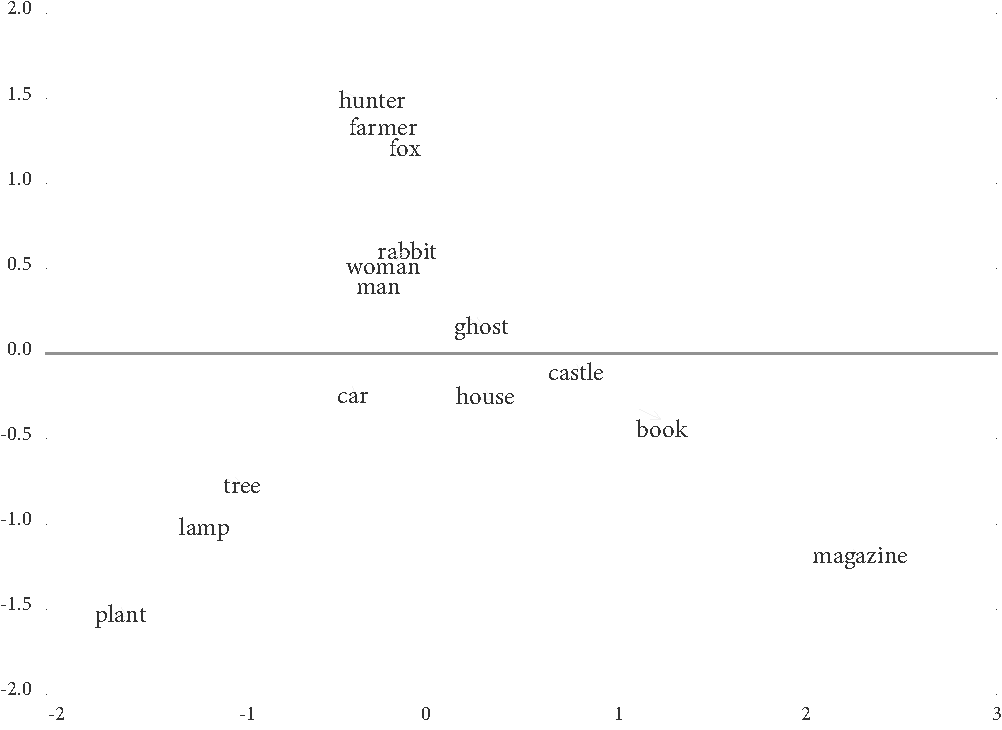
\includegraphics[width=0.7\textwidth]{images/pca-clean.pdf}
\caption[PCA projection of animate and inanimate words.]{Two-dimensional PCA projection of the 300 dimensional word embedding vectors for a number of animate and inanimate words. The horizontal line illustrates the separability between the two classes in the first dimension.}
\label{fig:pca}
\end{figure}

To give an illustration of this idea, Figure \ref{fig:pca} depicts a two-dimensio\-nal Principle Component Analysis (PCA) projection of the 300 dimensional word embedding vectors for a number of typically animate and typically inanimate words. The horizontal gray line in the plot illustrates the separability of the animate and inanimate words in the first dimension of the PCA projection. It is interesting to observe that \emph{ghost} is the one closest to all other inanimate entities. Likewise, words such as \emph{castle}, \emph{house} or \emph{car} are often used in figurative language (metonymy), for example to refer to the people owning or living in the castle. Perhaps this ambiguous animacy position is responsible for their position in the first dimension close to real animate entities.


\subsubsection{Models}\label{sec:animacy-models}
The model employs a Maximum Entropy classifier with L2 regularization as implemented in the Scikit-Learn Machine Learning Toolkit\autocite{sklearn:2011}. In all experiments, the regularization strength parameter $C$ is set to $C=1$.

I compare nine models which make use of different feature combinations: (1) words, (2) words and Part-of-Speech tags, (3) words, Part-of-Speech tags and lemmata, (4) words, Part-of-Speech tags, lemmata and dependency tags, (5) word embeddings and (6-9) the features in model 1 to 4 with word embeddings.

Although the background corpus is sufficiently large to cover most words in an unseen text, there will always be rare words for which the model does not have learned word embeddings. Therefore, in order to effectively make use of the word embedding vectors, we need a way to deal with out-of-vocabulary items. I adopt a simple strategy where I make use of a primary classifier and a back-off classifier. For models 6 to 9, I augment each word with its corresponding 300 dimension word embeddings vector. In the case of out-of-vocabulary words, the system resorts to a back-off model that contains all features except the word embeddings. For example, a model that makes use of words and word embeddings, will make a prediction on the basis of the word features alone. In case of the model that solely uses the embeddings (model 5), the back-off classifier is a majority vote classifier, which classifies unseen words as inanimate.

\subsubsection{Results}\label{sec:animacy-results}

Table \ref{tab:results-all} presents the results for all nine models on the complete data set. For each model I report the Precision, Recall and $F1$-score for animate words and inanimate words.

\begin{table}[t]
\centering
\begin{tabular}{lrrrrrr}
\toprule
                       & \multicolumn{3}{c}{inanimate} & \multicolumn{3}{c}{animate} \\ \midrule
model                  & Precision  & Recall & $F1$            & Precision  & Recall & $F1$  \\ \cmidrule(r){1-7}
1                      & 0.96 & 0.99 & 0.98            & 0.94 & 0.78 & 0.85  \\
2                      & 0.97 & 0.99 & 0.98            & 0.94 & 0.86 & 0.89  \\
3                      & 0.97 & 0.99 & 0.98            & 0.94 & 0.86 & 0.90  \\
4                      & 0.97 & 0.99 & 0.98            & 0.94 & 0.86 & 0.90  \\
5                      & 0.98 & 0.99 & 0.98            & 0.93 & 0.89 & 0.91  \\
6                      & 0.98 & 0.99 & 0.98            & 0.94 & 0.90 & 0.91  \\
\rowcolor{lightgray}7  & 0.98 & 0.99 & 0.99            & 0.94 & 0.91 & 0.93  \\
8                      & 0.98 & 0.99 & 0.99            & 0.94 & 0.91 & 0.93  \\
9                      & 0.98 & 0.99 & 0.99            & 0.94 & 0.92 & 0.93  \\
\bottomrule
\end{tabular}
\caption[Animacy classification results on the complete data set.]{Precision, Recall and $F1$-score for animate and inanimate classes per feature setting for all words. The table presents the results for the following nine models: \textbf{1}) words; \textbf{2}) words and Part-of-Speech tags; \textbf{3}) words, Part-of-Speech tags and lemmata; \textbf{4}) words, Part-of-Speech tags, lemmata and dependency tags; \textbf{5}) word embeddings; \textbf{6}) words and word embeddings; \textbf{7}) words, Part-of-Speech tags and word embeddings; \textbf{8}) words, Part-of-Speech tags, lemmata and word embeddings; \textbf{9}) words, Part-of-Speech tags, lemmata, dependency tags and word embeddings.}
\label{tab:results-all}
\end{table}

All models perform well on classifying inanimate words. However, since this is the majority class, it is of course far more interesting to compare the performance of the models on the animate instances. It is interesting to observe that the `simple' $n$-gram word model already performs rather well. Adding more features, such as Part-of-Speech, lemmata, etcetera, only has a positive impact on the recall of the model, while leaving the precision untouched. As can be observed from the table, employing the rather expensive dependency features shows barely any improvement.

\begin{table}[t]
\centering
\begin{tabular}{lrrrrrr}
\toprule
                      & \multicolumn{3}{c}{inanimate} & \multicolumn{3}{c}{animate} \\ \midrule
model                 & Precision  & Recall  & $F1$ & Precision  & Recall  & $F1$  \\ \cmidrule(r){1-7}
1                     & 0.78 & 0.98 & 0.87 & 0.96 & 0.60 & 0.74 \\
2                     & 0.86 & 0.96 & 0.90 & 0.93 & 0.78 & 0.84 \\
3                     & 0.87 & 0.96 & 0.91 & 0.94 & 0.80 & 0.86 \\
4                     & 0.87 & 0.96 & 0.91 & 0.93 & 0.80 & 0.86 \\
5                     & 0.90 & 0.96 & 0.92 & 0.93 & 0.85 & 0.89 \\
6                     & 0.90 & 0.97 & 0.93 & 0.95 & 0.85 & 0.90 \\
\rowcolor{lightgray}7 & 0.93 & 0.96 & 0.95 & 0.95 & 0.90 & 0.92 \\
8                     & 0.93 & 0.96 & 0.94 & 0.95 & 0.89 & 0.92 \\
9                     & 0.93 & 0.96 & 0.95 & 0.95 & 0.90 & 0.92 \\
\bottomrule
\end{tabular}
\caption[Animacy classification results on all (proper) nouns.]{Precision, Recall, and $F1$ score for animate and inanimate classes per feature settings for all words tagged as noun. The table presents the results for the following nine models: \textbf{1}) words; \textbf{2}) words and Part-of-Speech tags; \textbf{3}) words, Part-of-Speech tags and lemmata; \textbf{4}) words, Part-of-Speech tags, lemmata and dependency tags; \textbf{5}) word embeddings; \textbf{6}) words and word embeddings; \textbf{7}) words, Part-of-Speech tags and word embeddings; \textbf{8}) words, Part-of-Speech tags, lemmata and word embeddings; \textbf{9}) words, Part-of-Speech tags, lemmata, dependency tags and word embeddings.}
\label{tab:results-noun}
\end{table}

The model that only uses word embedding features is one of the best performing models. This is a context-insensitive model that operates on the level of the vocabulary, which means that it will predict the same outcome for each token of a particular word type. The high precision and high recall show us that this model has acquired knowledge about which words \emph{typically} group with animate words and which with inanimate words. However, the models that combine the word embeddings with the context sensitive features, such as word $n$-grams or Part-of-Speech tags, outperform the context-insensitive model.

The best performance is achieved by the model that combines the word features, part-of-speech tags and the word embeddings, which has an $F1$-score of 0.93 on animate words and 0.99 on inanimate words. Adding more features does not result in any more performance gain. Table \ref{tab:results-noun} presents the results for all nouns and names in the data set. The best performance is again achieved by the model that combines the word features with the part-of-speech tags and word embeddings, resulting in an $F1$-score of 0.92 for animate instances and 0.95 for inanimate instances. Recall from Section \ref{sec:animacy-data} that being a noun or proper name already is an indication for animacy. This could explain the somewhat lower scores for the inanimate class.

\subsection{Experiment 2}\label{sec:animacy-exp-2}

The approach to animacy classification presented in Experiment 1 appears to be successful. In the current section, I employ the classification system to extract all animate entities from unannotated folktales from the Dutch Folktale Database, all of which were not used in the previous experiment.\footnote{\url{http://www.verhalenbank.nl}} First, it allows us to further the evaluation of the classifier. In a classical evaluation setup -- as with the above-described approach -- general practice is to train a computational system on some training data. The performance of the system is then evaluated on a held-out test set. Even if we include a separate development set, this setup could run the risk of `overfitting' the data. The annotated corpus contains a reasonably diverse set of stories in terms of genre, yet it is fairly small and rather homogeneous in style. Even though I performed a cross-validation experiment, there is a chance of `overfitting' to the style of the subset of folktales trained on. 

\subsubsection{Data Collection}
For the evaluation I make use of a subcollection of folktales from the Dutch Folktale Database. The complete collection consists of about 44,000 folktales\autocite{meder:2010,meder:2016}, and contains stories from various genres (e.g.\ fairytales, legends, urban legends, jokes, personal narratives) in standard Dutch and Frisian, as well as a number of dialectal variants. Every entry in the database contains meta-data about the story, including language, collector, place and date of narration, keywords, names, and subgenre. Here, I make use of a subcollection comprising 16,294 stories written in Standard Dutch. The distribution of genres in the subcollection is the following: urban legends ($n=2795$), legends ($n=299$), jokes ($n=3986$), personal narratives ($n=693$), riddles ($n=1626$), sagas ($n=6045$) and fairy tales ($n=832$). I evaluate a random sample of this subcollection ($n=212$) in which this genre distribution is taken into account.

\begin{figure}
\centering
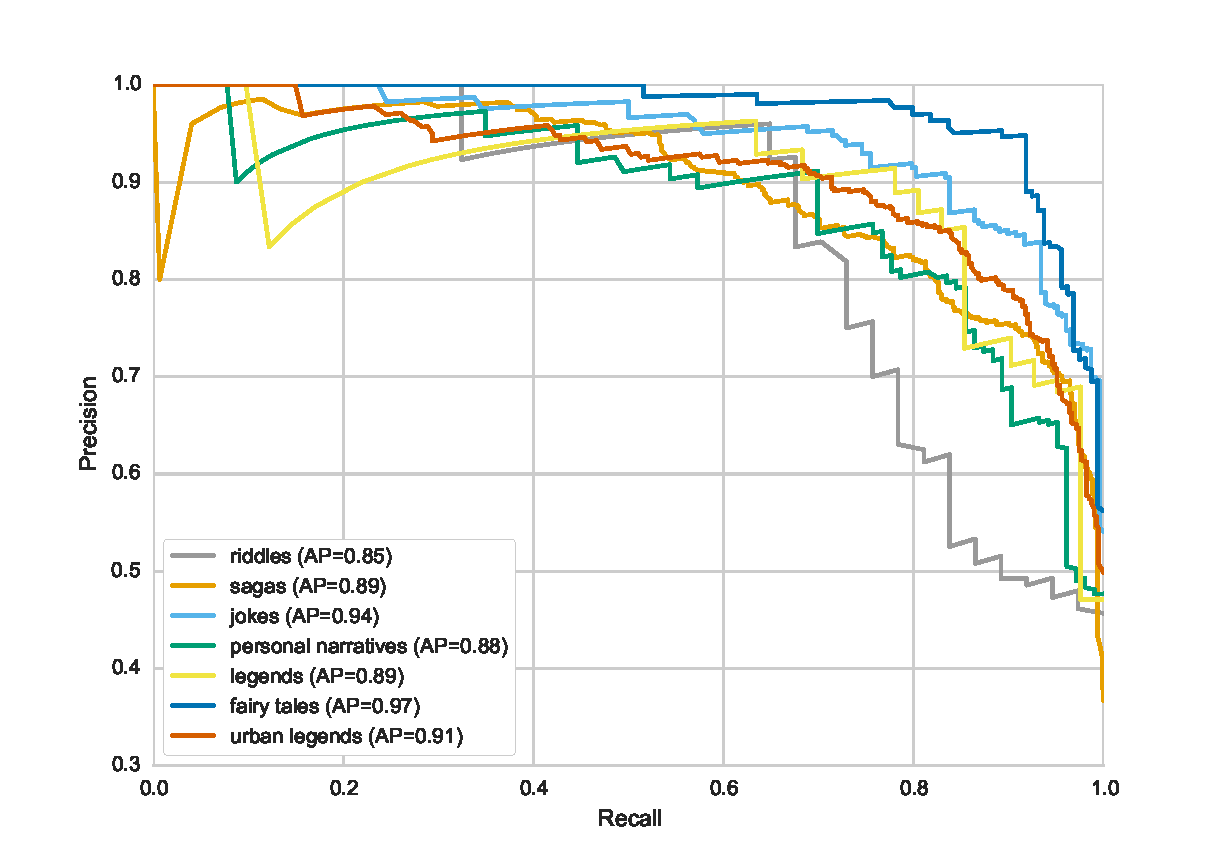
\includegraphics[width=\textwidth]{images/precision-recall-curve}
\caption{Precision-Recall Curves and Average Precision scores per genre.}
\label{fig:prec-recall-curve}
\end{figure}

\subsubsection{Task Description}
The proposed definition of animacy allows us to utilize the animacy detection system to extract all characters from a story in a similar vein as \citeauthor{karsdorp:2012b}.\autocite{karsdorp:2012b} The system labels each noun and name in a text for animacy. After removing duplicate words, this produces a set of words that comprises the cast of a story. Without golden standard annotations, however, these character sets can only be evaluated for precision and not for recall. I therefore take an alternative approach, in which for each story I produce a ranking of all its words. The goal here is to allocate the highest positions in these rankings to animate entities. 

\subsubsection{Evaluation}
Formulating the task as a ranking problem allows us to evaluate the rankings by means of the \emph{Average Precision} score, which computes the average over precision scores at increasing points of recall:
\begin{equation}
\text{AP} = \frac{\sum^n_{k=1} (P(k) \times \text{rel}(k))}{\text{number of relevant items}},
\end{equation}
where $\text{rel}(k)$ equals 1 if the item at rank $k$ is an actual character, zero otherwise, and $P(k)$ represents the precision at cut-off $k$. Naturally, with this evaluation method, the rankings still need to be manually evaluated. By using a rank cutoff and evaluating a sample of all automatically annotated stories, the costly manual labor is reduced to a minimum. All nouns and names in a story are ordered based on the output of the probabilistic decision function of the Maximum Entropy classifier which was used in Experiment 1. After removing duplicate words, this produces a final ranking. The rankings are evaluated with a rank cut-off at 50.

\subsubsection{Results}
Figure \ref{fig:prec-recall-curve} presents the Precision-Recall curve as well as the \emph{Average Precision} score for each genre. The Precision-Recall curve is obtained from computing precision-recall pairs for different probability thresholds. The system performs well, especially on fairy tales ($\text{AP}=0.97$) and jokes ($\text{AP}=0.94$).\footnote{An AP of 0.97 means that on average, nearly all actual cast members of a folktale are ranked on top, with the first case of a non-animate entity entering the ranking at about rank 5 or 6 on average.} The lowest performance is measured on riddles ($\text{AP}=0.85$). This lower score is mainly the result of the system's inability to position the word \emph{blondje} (`dumb blond' with a pejorative connotation, which is prevalent in the so-called `dumb blond jokes') high up the ranking.

\subsection{Conclusion}

The proposed approach to create a model for animacy classification using linguistically uninformed features proves to be successful. I compared the performance of linguistically informed models (using features such as part-of-speech and dependency tags) to models that make use of lower-dimensional, semantic representations of the data. With the exception of the model that solely makes use of these representations, all models benefit from adding these semantic features. The model that requires the least linguistic information (word $n$-grams plus word embeddings) outperforms all linguistically informed models (without embeddings). The best results are reported by the model that combines word $n$-grams with part-of-speech $n$-grams and word embeddings.

\section{Character Type Selection Bias in Fairy Tales}\label{sec:grimmpopularity}

In this section I will return to the central questions set out in the introductory section \ref{sec:cultural-success-intro}. My aim is to further explore and build on \citeauthor{joosen:2014}'s observation that the present-day fairy tale canon is dominated by female protagonists\autocite{joosen:2014}, and more thoroughly investigate the more general question of whether cultural selection and successfulness of fairy tales involves biases towards or \emph{away} from tales that revolve around particular character types. This question will be addressed through a systematical examination of the character cast retrieved from the fairy tales in the 1857 edition of the Grimm's \emph{Kinder- und Hausmärchen}. As will be explained in more detail in Section \ref{sec:grimm-collection}, the 210 tales in \emph{Kinder- und Hausmärchen} exhibit varying degrees of successfulness. In Section \ref{sec:character-typology}, then, I apply the animacy detection model (set out in Section \ref{sec:animacy}) to the Grimm's fairy tales collection, and map out the yielded character lists to a computationally induced folktale character typology. Subsequently, I assign a character type to each of the characters in the Grimm's fairy tale collection, which enables us to employ statistical methods to assess which character types are distinctively associated with either successful or unsuccessful tales (Section \ref{sec:popularity-results}).

\subsection{Data Collection}\label{sec:grimm-collection}

The object of study is the Dutch translation of the Brothers Grimm's 1857 edition of \emph{Kinder- und Hausmärchen} by \citeauthor{Vries-Vogel:1984} from \citeyear{Vries-Vogel:1984}.\autocite{Vries-Vogel:1984} The complete collection comprises 210 tales, including nowadays highly popular ones, such as ``Cinderella'' and ``Hansel and Gretel'', but also many tales that are relatively unknown, such as ``The Prince Who Feared Nothing'' and ``Maid Maleen''. Following \citeauthor{Norenzayan:2006}, each of the collection's tales were considered as popular or impopular based on their position on a popularity index.\autocite{Norenzayan:2006} In this index, the popularity of fairy tales is measured through web page hits obtained from the search engine Google. \citeauthor{Norenzayan:2006} propose the following division of successful as opposed to unsuccessful tales:

\begin{description}
\item[Culturally successful ($N = 21$):]
{``The Frog King'' (``Iron Henry'') (1), ``Little Brother and Little Sister'' (11), ``Rapunzel'' (12), ``Hansel and Gretel'' (15), ``The Fisherman and his Wife'' (19), ``The Brave Little Tailor'' (20), ``Ashputtle'' (``Cinderella'') (21), ``Mother Holle'' (24), ``Little Red Cap'' (``Little Red Riding Hood'') (26), ``The Musicians of Bremen'' (27), ``The Devil with the Three Golden Hairs'' (29), ``Little Brier Rose'' (``Sleeping Beauty'') (50), ``King Thrushbeard'' (52), ``Snow White'' (53), ``Rumpelstiltskin'' (55), ``Thousandfurs'' (65), ``Jorinde and Joringel'' (69), ``Hans in Luck'' (83), ``The Singing, Springing Lark'' (``Beauty and the Beast'') (88), ``The Goose Girl'' (89), ``Snow White and Rose Red'' (161).}

\item[Culturally unsuccessful ($N = 21$):]
``A Good Stroke of Business'' (7), ``The Girl Without Hands'' (31), ``The Magic Table, The Gold Donkey, and the Cudgel in the Sack'' (36), ``The Knapsack, the Hat, and the Horn'' (54), ``Frederick and Liza-Kate'' (59), ``Farmer Little'' (61), ``Six Who Made Their Way in the World'' (71), ``The Carnation'' (76), ``Brother Scamp'' (81), ``The Golden Children'' (85), ``The King of the Golden Mountain'' (92), ``The Spirit in the Bottle'' (99), ``Bearskin'' (101), ``Hans My Hedgehog'' (108), ``The Jew in the Brambles'' (110), ``The Prince Who Feared Nothing'' (121), ``The Donkey Lettuce'' (122), ``Faithful Ferdinand and Faithless Ferdinand'' (126), ``Hefty Hans'' (166), ``The Poor Boy in the Grave'' (185), ``Maid Maleen'' (198).
\end{description}

\noindent Although these lists were compiled on the basis of English and German web page hits, the list of successful tales shows a strong correlation with popularity polls in the Dutch language area.\footnote{I.e.\ the top seven tales in the popularity poll executed by \citeauthor{koman:2008} are all included in the `successful group' (``Snow White'' (53), ``Cinderella'' (21), ``Sleeping Beauty'' (50), ``Little Red Riding Hood'' (26), ``Hansel and Gretel'' (15), ``Rumpelstiltskin'' (55) and ``The Beauty and the Beast'' (88)).} For reasons of comparability, then, I will adopt \citeauthor{Norenzayan:2006}'s classification of successful (i.e.\ popular) and unsuccessful (i.e.\ impopular) tales in this study.

\begin{figure}[t]
\centering
\subfigure[Density plot and histogram of the number of characters per story.]{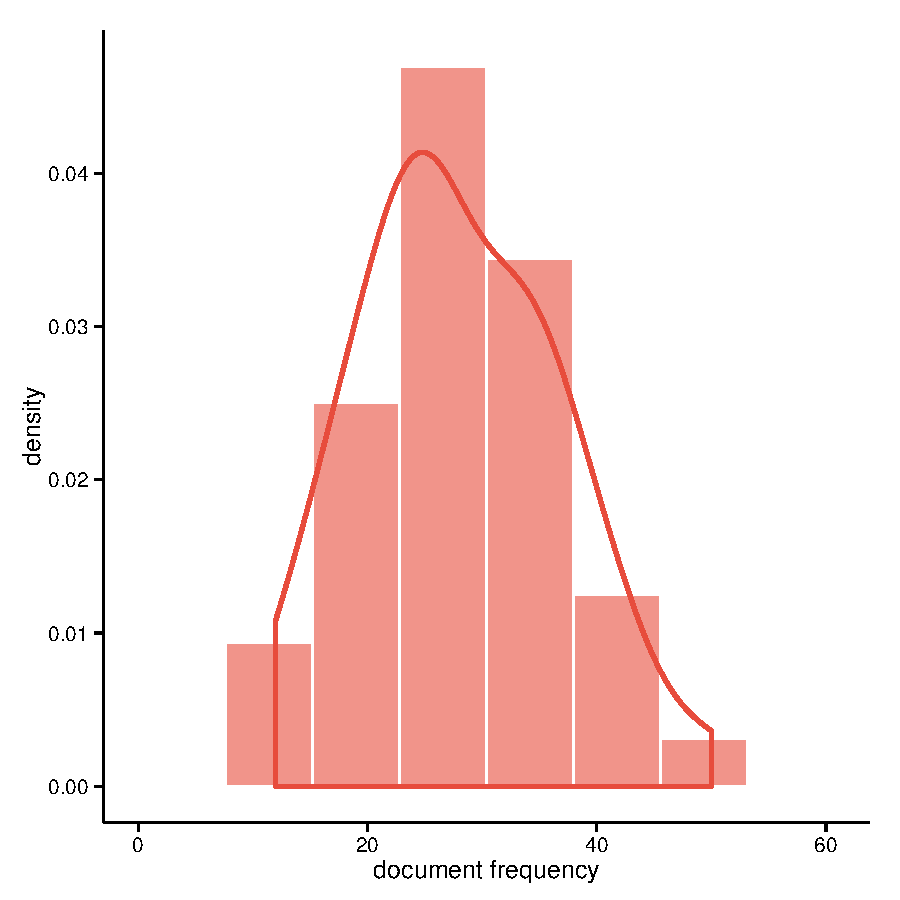
\includegraphics[width=0.49\textwidth]{images/grimm-char-fd.pdf}}
\subfigure[CCDF of character document frequency.]{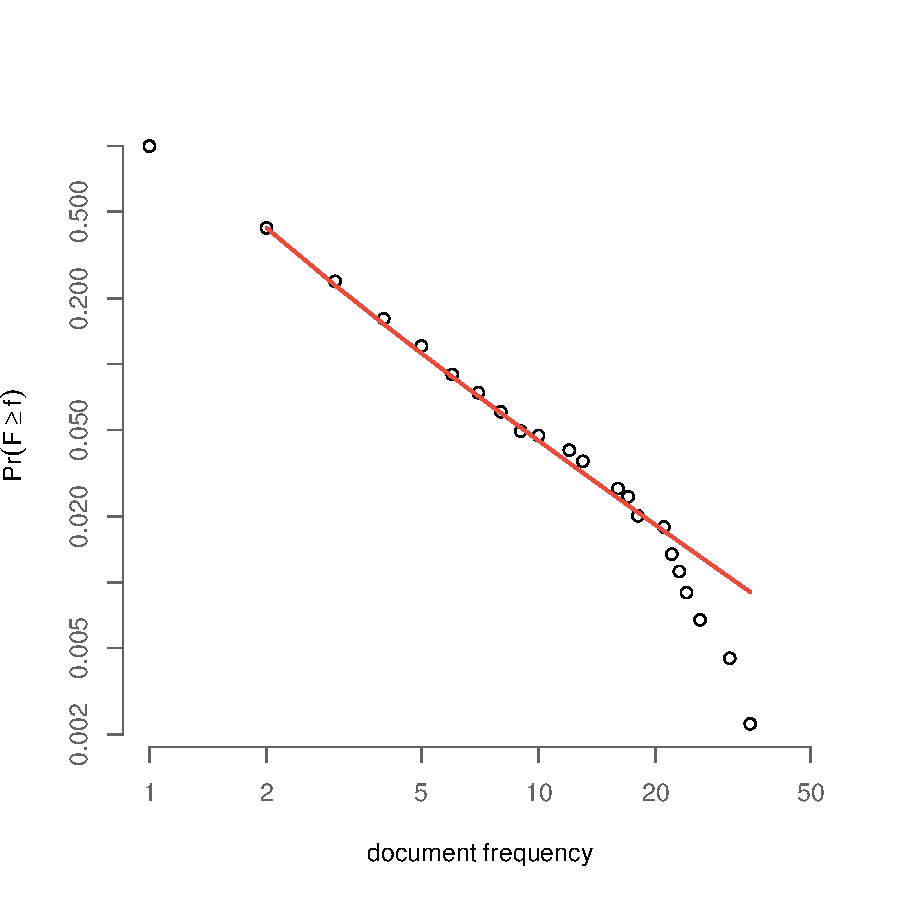
\includegraphics[width=0.49\textwidth]{images/grimm-pl.pdf}}
\caption{The left subplot (a) displays a density plot and histogram computed over the number of unique characters per story in the $N=42$ sub-collection of the Brother's Grimm. The right subplot displays the complementary cumulative frequency distribution of the character story frequency.}
\label{fig:grimm-character-statistics}
\end{figure} 

Each of the 42 tales in this collection were submitted to the animacy detection system, which yields a list of characters for each story. After a manual filtering of all classification errors and animate entities of which the syntactic category is not a (proper) noun, we obtain a list of 1,177 characters and 446 unique character types in total. On average, each tale mentions about 28 characters ($\sigma=8.63$). Note that this number not necessarily concurs with the actual number of characters in a story, because I did not attempt to resolve any co-references, and multiple words may refer to the same unique character in a story. As can be observed from Figure \ref{fig:grimm-character-statistics}(a), the number of characters per story is rather normally distributed. When we investigate the frequency distribution of the characters, we find that a large proportion of characters occurs only in a few stories or in a single story and only a few yet significant number of characters occur in many different stories. In fact, according to the bootstrap procedure proposed by \citeauthor{clauset:2009}, the distribution exhibits a good fit $(p=0.7)$ to a power-law model with an exponent of $\alpha=2.24$ (cf.\ Figure \ref{fig:grimm-character-statistics}(b)).\autocite[See][and Chapter 5 for a more in depth explanation of power-laws and the bootstrap procedure.]{clauset:2009}


\subsection{Character Typology}\label{sec:character-typology}

Let us now consider the question whether successful tales revolve around character types that are distinctively different from the character set in unsuccessful tales. In order to address this question, we first need to establish a mapping between each unique retrieved character and a particular character type. A character type is defined as a semantically and/or functionally coherent group of characters. The agglomeration of all character types constitutes a folktale character typology, onto which the unique characters in the Grimm's tales will eventually be mapped. To create this typology, I used the list of folktale characters that have been extracted from the Dutch Folktale Database in Section \ref{sec:animacy-exp-2}. The classification errors, duplicates and all entities that occur less than a thousand times in COW were removed, yielding a list of 4,548 unique characters. Rather than manually developing a character typology -- which is both labor-intensive as well as prone to subjective assessments -- I choose to construct a character typology by means of an automatic procedure, in which character types are formed by means of a cluster algorithm.

\begin{figure}
\centering
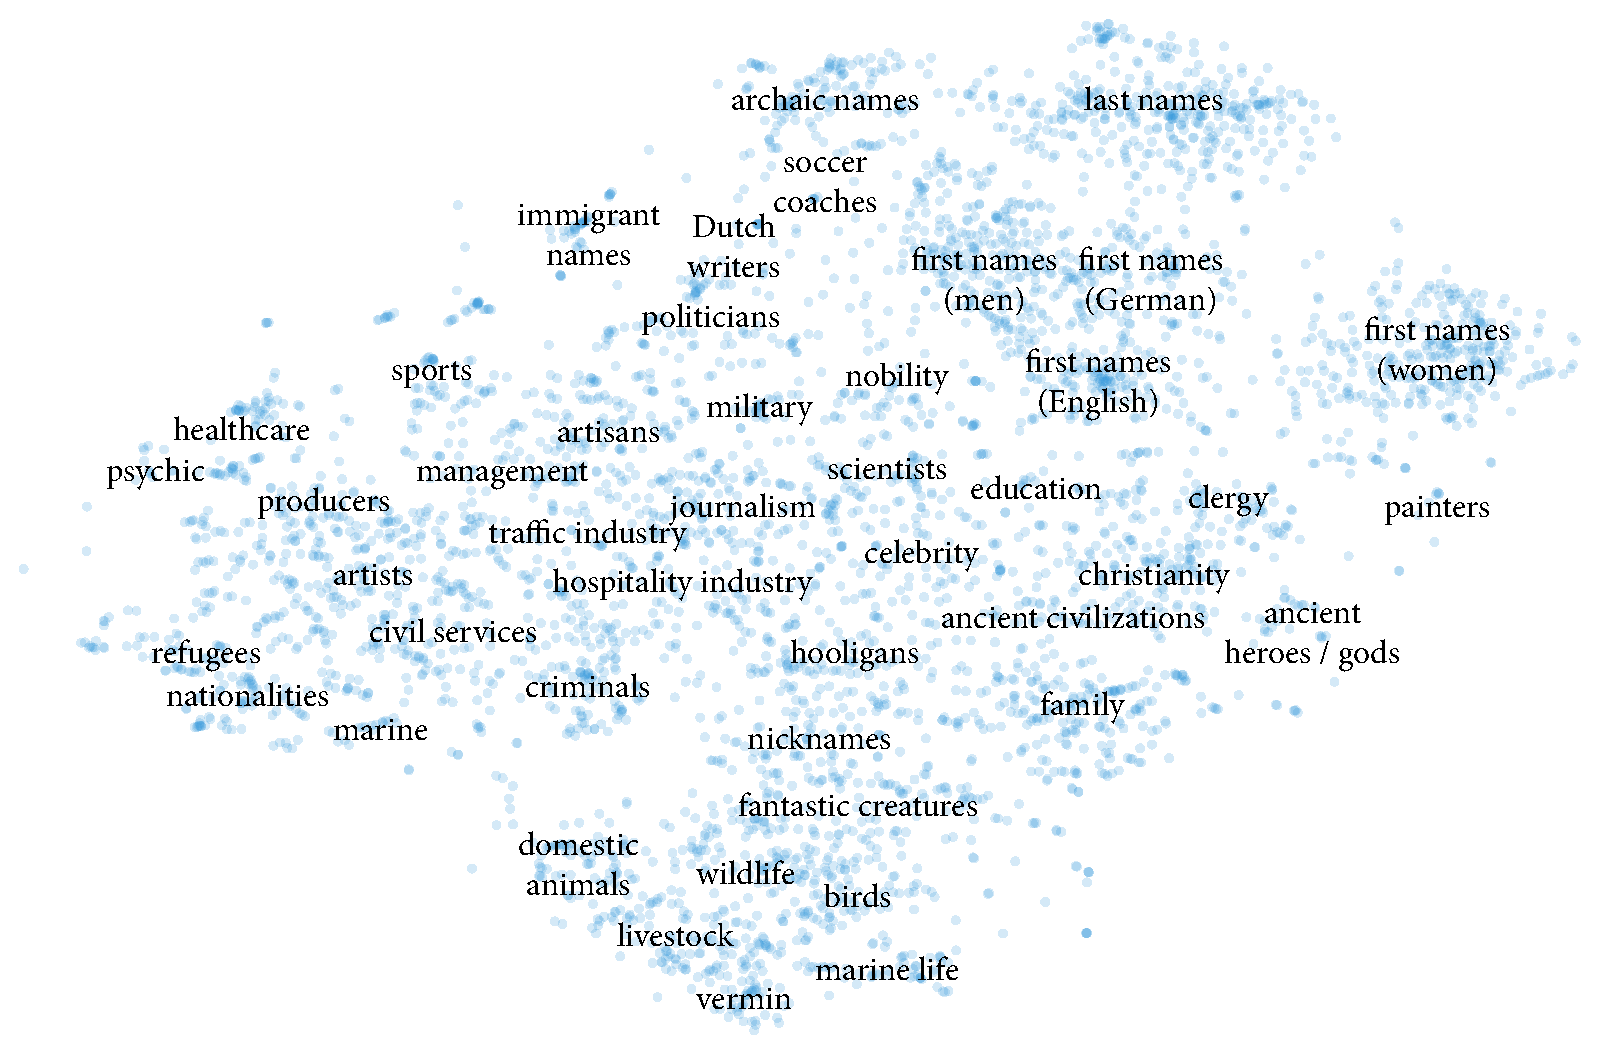
\includegraphics[width=\textwidth]{images/character-map.pdf}
\caption{Visualization of the characters extracted from Dutch stories of the Dutch Folktale Database based on their word embeddings using t-SNE.}
\label{fig:animacy-character-map}
\end{figure}

The word embeddings that are used as features in the animacy classifier can be employed to describe the similarities and dissimilarities between the extracted animate entities. Figure \ref{fig:animacy-character-map} presents a two-dimensional semantic map that depicts the (dis)similarities between all extracted animate entities.\footnote{Readers are invited to view an interactive version of the map at the following web-address: \url{fbkarsdorp.github.io/animacy-detection}.} The dimension reduction was performed using t-Distributed Stochastic Neighbor Embedding (t-SNE)\autocite{maaten:2008}. The map discloses a rich diversity of animate entities grouped into highly semantically coherent clusters. The cluster at the bottom of the map, for example, represents a grouping of all kinds of animals. This cluster comprises manifold subtle sub-clusters describing more specific positions in the animal taxonomy, e.g.\ birds and livestock, marine life, vermin, wildlife, and domestic animals. The groupings to the left are occupied by characters of different professions. There is a large number of characters from the hospitality industry (e.g.\ waiter and cook), as well as from the transport sector (e.g.\ chauffeur and train conductor), and from health-care services (e.g.\ doctors, patients, and surgeons).

Another cluster worth mentioning is the one that is occupied by characters from Christianity. This cluster is noteworthy because, like the animal cluster, it is clearly structured into various hierarchically ordered clusters with several emerging subgroups. One subgroup entails religious or even Christian professions, such as `bishops' and `vicar'. From there, a link via `catholics' and `protestants' leads to the more general `believers' and `followers'. This mini-node bifurcates into two different nodes. First, we find a cluster containing words designating followers of different religions, such as `Jew' and `Muslim'. This cluster branches off to a `religious fringe' node, containing `cult', `satanist' and `Freemasons'. The other cluster connected to the mini-node of `believers' and `followers' is structurally complex, starting with such terms as `people' and `believers' but continuing through `Satan' and `Lucifer' to `angels' and `guardian angels'. These words form again a bridge towards more esoteric creatures, such as `nature spirits'. Numerous other groupings can be discerned in Figure \ref{fig:animacy-character-map}, ranging from broad categories, such as `fantastic creatures', `criminals' and `hooligans', to more specialized clusters such as the one containing soccer coaches or people with psychic abilities (e.g.\ `clairvoyants', `mediums' and `fortune-tellers'). 

Combined with the strength of t-SNE to position the characters on a two-dimensional map, the word embeddings yield a powerful representation. However, if we want to assign a character type to each character extracted from the fairy tales by the Brothers Grimm, we need to `hard-cluster' the characters into $k$ types. The above description is only part of the extremely rich network of associations this semantic map displays. Therefore, popular clustering algorithms such as $k$-means seem less suitable as they require to fix the number of clusters $k$ in the data upfront, which is far from straightforward to do. To circumvent the problem of cherry-picking $k$, I employ the cluster algorithm DP-means as proposed by \citeauthor{Kulis:2012}, which is a non-parametric Bayesian variant of the $k$-means algorithm and based on a Dirichlet Process mixture model\autocite{Kulis:2012}. The algorithm behaves similarly to $k$-means, yet it does not require that $k$ is fixed upfront, but it dynamically forms new clusters depending on whether the minimal distance between a data point and any of the existing centroids exceeds the threshold parameter $\lambda$. 

\begin{sidewaysfigure}
\centering
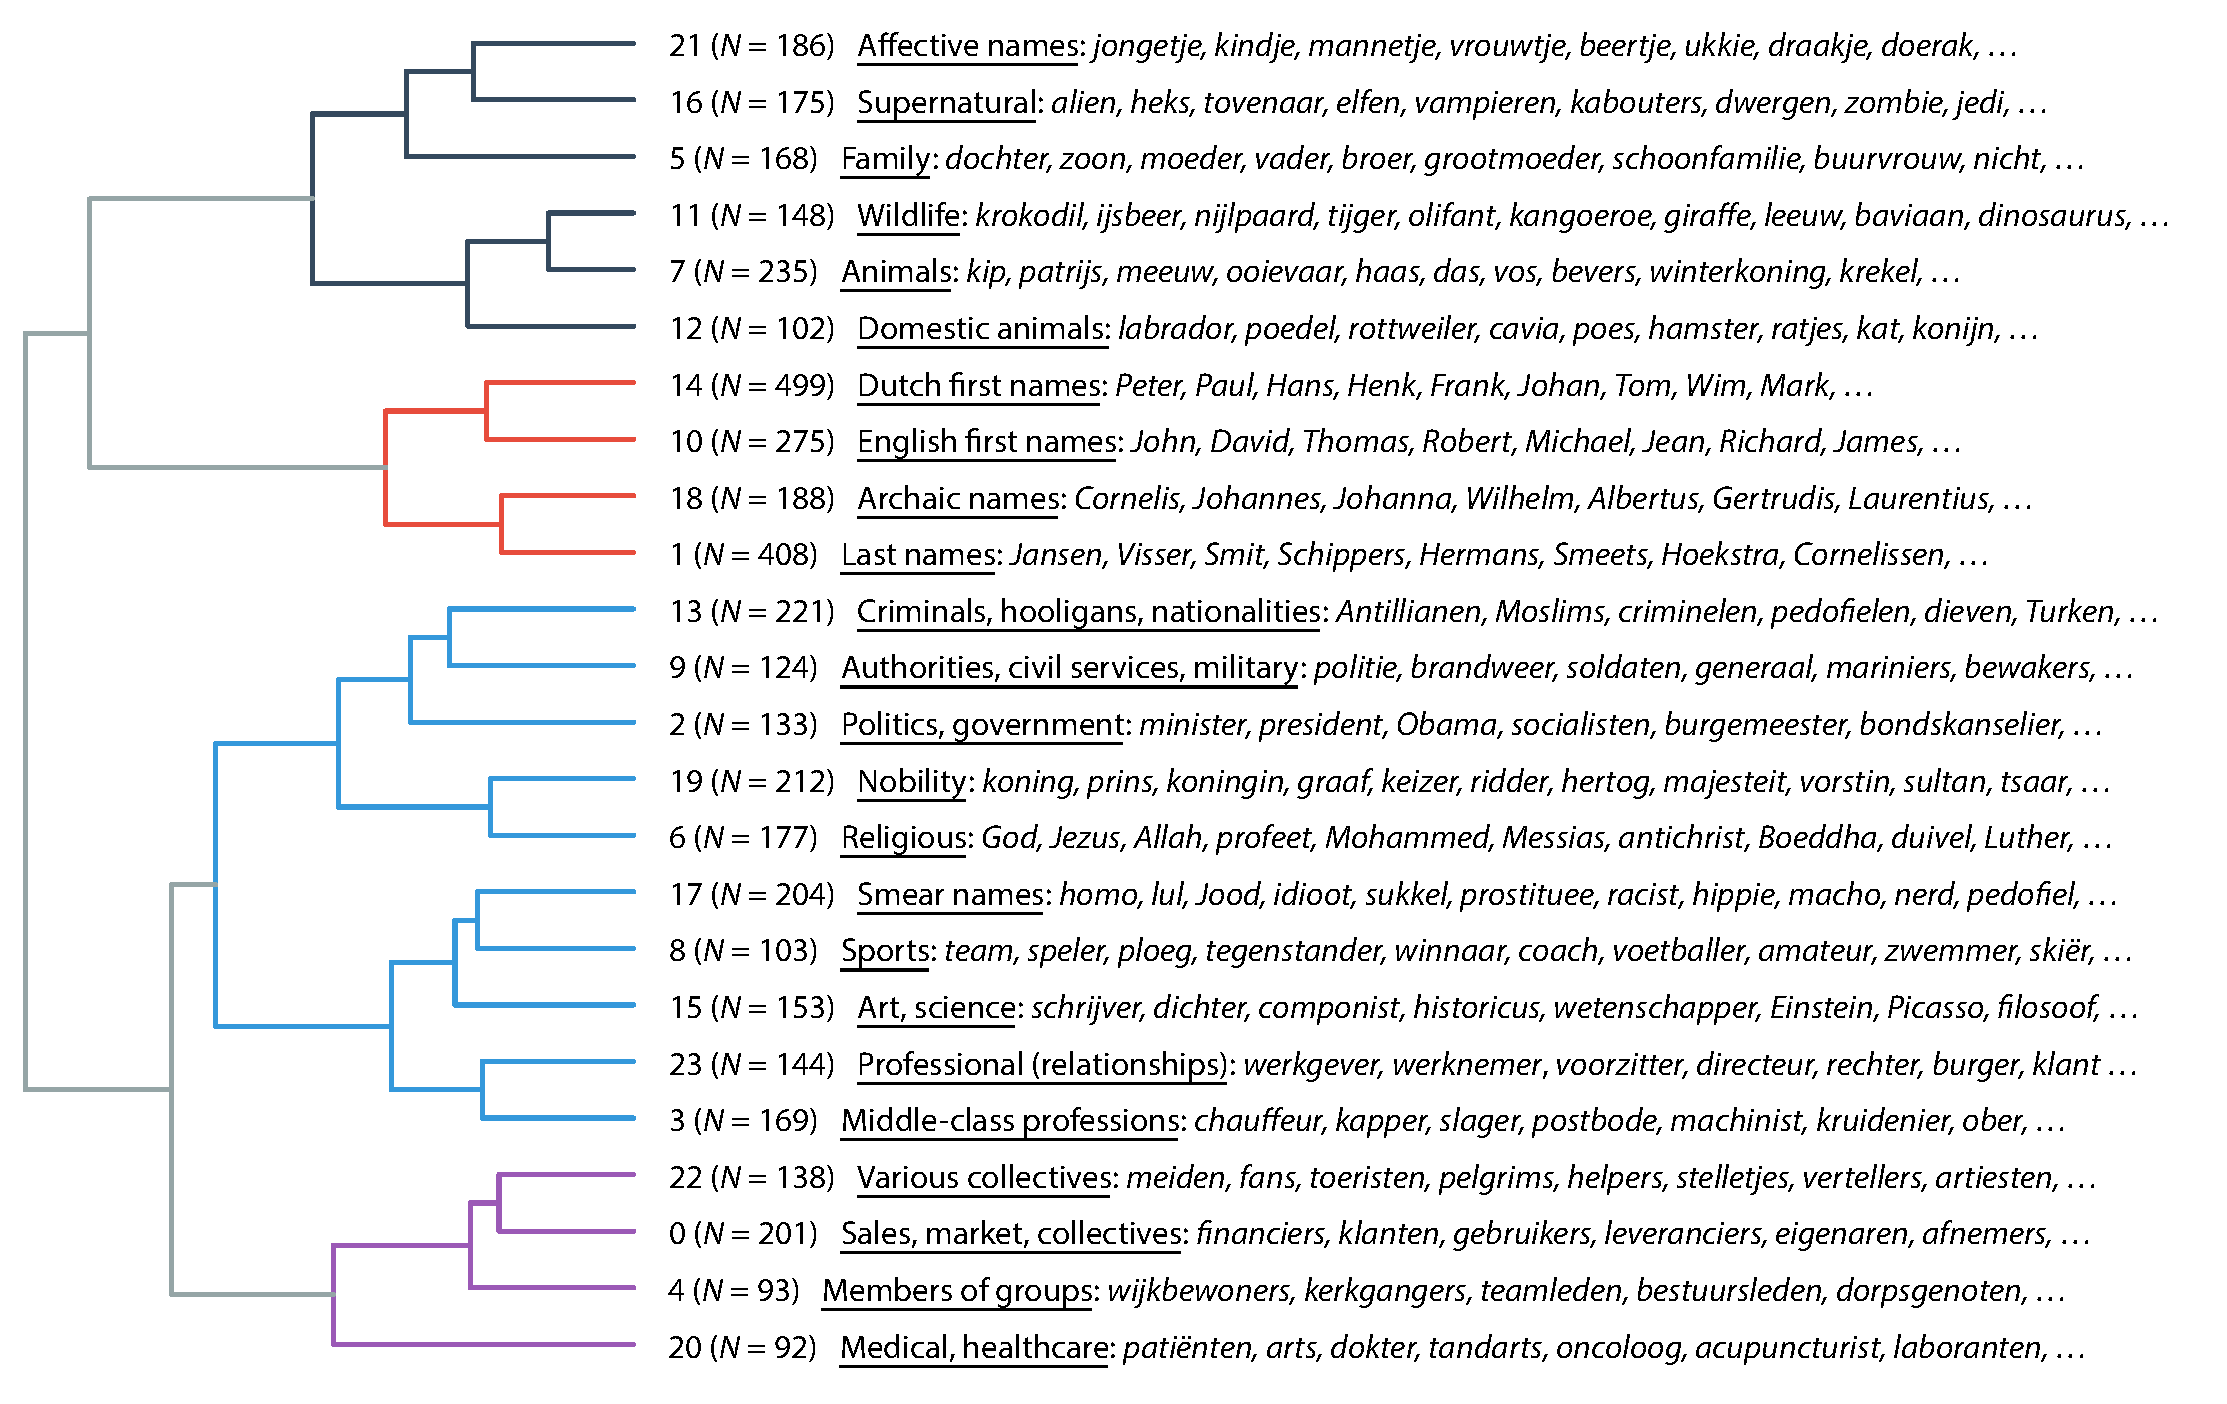
\includegraphics[width=\textwidth]{images/character-tree.pdf}
\caption{Hierarchical cluster tree of the 24 induced character types.}
\label{fig:animacy-cluster-map}
\end{sidewaysfigure}

Other than the $k$-means algorithm, which depends on the initial clustering of the data, the order in which the data is presented to the DP-means algorithm potentially has a severe impact on the resulting clustering. Under the assumption that the quality of word embeddings is higher for words that occur more frequently, I present the data to the cluster algorithm ordered by word frequency in COW in descending order. Note that the cluster penalty parameter $\lambda$ of DP-means controls for the specificity of the character types with lower values typically producing a larger number and also more detailed character types. In order to keep the typology manageable for interpretation and to reduce the risk of overfitting the data, I choose to set $\lambda$ at the rather conservative value of 0.7. The algorithm was set to run for 200 iterations. Under these settings, the algorithm produced the 24 clusters depicted in Figure \ref{fig:animacy-cluster-map}. The hierarchical tree was computed on the basis of the cosine distances between the centroid representations learned by DP-means.

Similar to the character map in Figure \ref{fig:animacy-character-map}, the cluster tree discloses multiple semantically coherent clusters of characters. Clusters 11, 7 and 12, for example, deal with various animals, which are grouped under `wildlife' (e.g.\ `lion', `hippopotamus', `crocodile'), `animals' (e.g.\ `chicken', `stork', `hamster') or `domestic animals' (e.g.\ `poodle', `guinea pig', `rabbit'). Another example is the red subtree, which represents an abstract cluster of proper names and entails four sub-clusters with first or last names from different nationalities. The upper subtree branches off into three clusters consisting of `affective names' (e.g.\ `little boy', `rascal', `little kid'), `supernatural entities' (e.g.\ `witch', `wizard', `elves') and `family related names' (e.g.\ `daughter', `brother', `mother'). The above-mentioned grouping of religious characters (predominantly from Christianity) is found in cluster 6, which is connected to cluster 19 consisting of various nobility characters, such as `duke', `king', `queen', and `prince'. 


\subsection{Results}\label{sec:popularity-results}

\begin{figure}
\centering
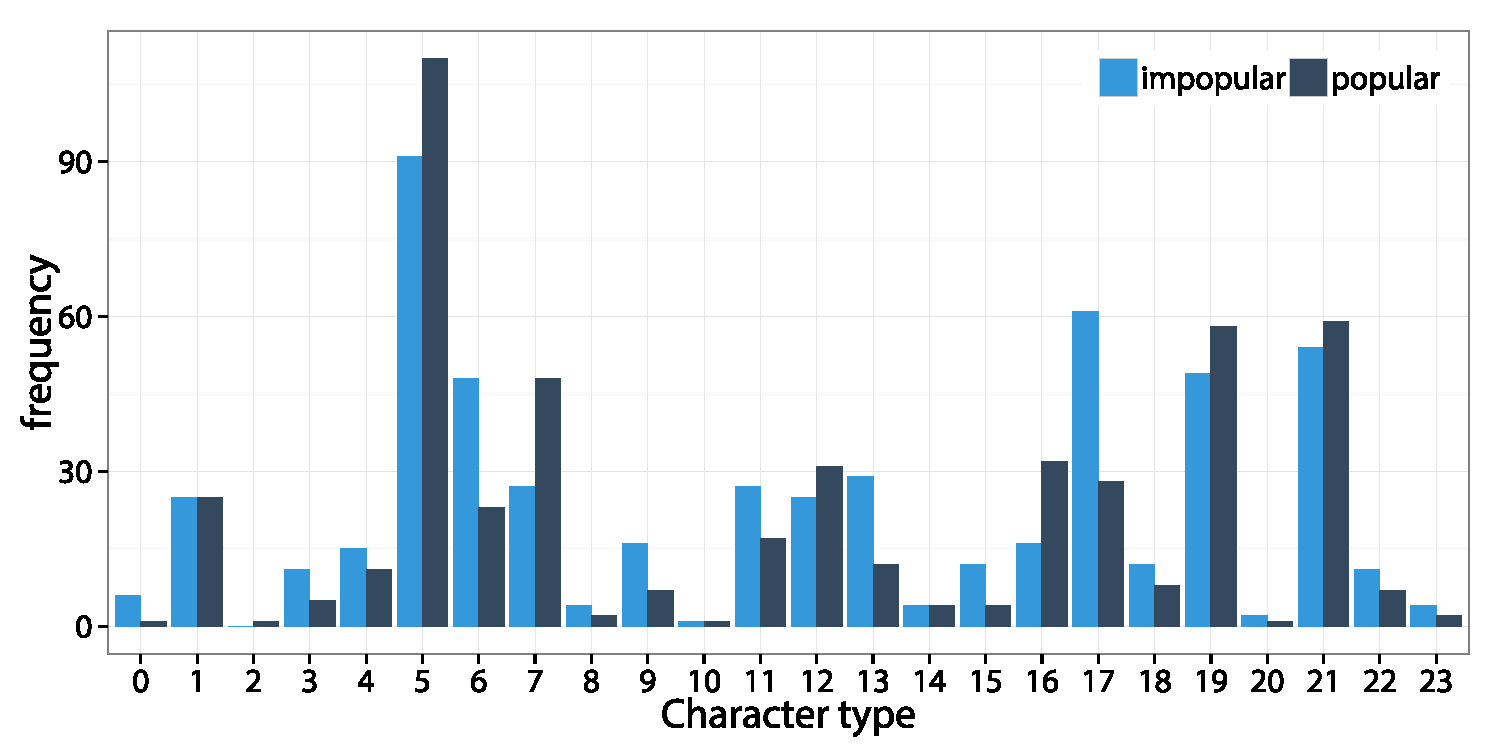
\includegraphics[width=\textwidth]{images/character-type-distribution.pdf}
\caption{Distribution of character types for successful and unsuccessful $N=42$ fairy tales from \emph{Kinder- und Hausmärchen} (1857) by the Brothers Grimm.}
\label{fig:character-type-distribution}
\end{figure}

The character typology discussed in the previous section serves as the methodological base for the main research question of this chapter on character type biases in story transmission. All characters extracted from the Brothers Grimm's fairy tale collection were mapped to a type in the character typology. Figure \ref{fig:character-type-distribution} displays the distribution of the character types for both successful and unsuccessful tales. It can be observed from the plot that character type 5, which deals with family relationships, dominates both successful and unsuccessful tales, with a preference for popular tales. We find, furthermore, that the religious character type (6) appears to be more frequently used in unsuccessful than in successful tales. Successful tales, by contrast, display a preference for animal characters (type 7). Although frequency counts such as these are insightful and suggestive, to address the question of whether particular characters display \emph{significant} preferences for either successful or unsuccessful fairy tales, we need, however, a more rigorous and statistically sophisticated approach. 

The approach I propose aims to quantify whether a particular character type is distinctively associated with either successful or unsuccessful fairy tales by means of Fisher's exact test\autocite{fisher:1922}. Starting from the null hypothesis that the successfulness of tales and a particular character type are independent from each other, we aim to detect deviations from this null hypothesis, which are indicative for statistically significant distinctive character types. Fisher's exact test has several advantages over other quantities and statistical tests that can be employed to measure association strengths between binomial variables (e.g.\ $\chi^2$-test, pointwise mutual information\autocite{church:1990} or Dunning's log-likelihood coefficient\autocite{dunning:1993}). One of the most important characteristics for my purposes, is that being an exact test, Fisher's exact test makes no assumptions about the distribution of the data and provides exact values even for very small sample sizes. 

\begin{table}
\centering
\begin{tabular}{lrrr}
\toprule
                   & character type 5 & other types & row totals \\ \midrule
successful tales   & 110    & 387         & 497        \\
unsuccessful tales & 91     & 459         & 550        \\
column totals      & 201    & 846         & 1047       \\
\bottomrule
\end{tabular}
\caption{The distribution of character type 5 in successful and unsuccessful fairy tales from \emph{Kinder- und Hausmärchen} (1857) by the Brothers Grimm.}
\label{tab:fisher-example}
\end{table}

To compute the distinctiveness of a particular character type for successful or unsuccessful tales, the following frequencies need to be collected: (a) the frequency of the character type in successful tales, (b) the frequency of the character type in unsuccessful tales, the summed frequency of all other character types (i.e.\ the total number of characters minus the frequency of the target character type) in both successful tales (c) and unsuccessful tales (d). These numbers, then, can be entered in a $2 \times 2$ contingency table and submitted to the Fisher exact test. To illustrate the procedure, in Table \ref{tab:fisher-example} I provide the required frequencies for character type 5 which deals with family relationships. Character type 5 occurs 110 times in successful tales and 91 times in unsuccessful tales. There are $497 - 110 = 387$ characters with a different character type in successful tales and $550 - 91 = 459$ differently classified characters in unsuccessful tales. Submitting these numbers to Fisher's exact test returns a rather small $p$-value of 0.013. This number tells us that the probability of observing this or an even more imbalanced ratio by chance is about 1.2\%. Since this number is well below the commonly used significance level of 5\%, we can safely conclude that the observed imbalance is statistically significant; successful tales revolve significantly more often around family characters than unsuccessful tales.

\begin{table}
\centering
\newcolumntype{R}{>{\raggedleft\arraybackslash}X}%
\begin{tabularx}{\textwidth}{lrRlRR}
\toprule
type &  unsuccessful &  successful & preference & odds & $p$ \\
\midrule
0  &  6 &   1 &  unsuccessful &  5.471 &  0.080 \\
1  & 25 &  25 &     --   &  0.899 &  0.696 \\
2  &  0 &   1 &    successful &  0.000 &  0.475 \\
3  & 11 &   5 &  unsuccessful &  2.008 &  0.145 \\
4  & 15 &  11 &  unsuccessful &  1.239 &  0.370 \\
\rowcolor{lightgray}5  & 91 & 110 &    successful &  0.698 &  0.013 \\
\rowcolor{lightgray}6  & 48 &  23 &  unsuccessful &  1.971 &  0.006 \\
\rowcolor{lightgray}7  & 27 &  48 &    successful &  0.483 &  0.002 \\
8  &  4 &   2 &  unsuccessful &  1.813 &  0.392 \\
9  & 16 &   7 &  unsuccessful &  2.097 &  0.073 \\
10 &  1 &   1 &     --   &  0.903 &  0.775 \\
11 & 27 &  17 &  unsuccessful &  1.458 &  0.148 \\
12 & 25 &  31 &    successful &  0.716 &  0.141 \\
\rowcolor{lightgray}13 & 29 &  12 &  unsuccessful &  2.250 &  0.012 \\
14 &  4 &   4 &     --   &  0.903 &  0.691 \\
15 & 12 &   4 &  unsuccessful &  2.749 &  0.057 \\
\rowcolor{lightgray}16 & 16 &  32 &    successful &  0.435 &  0.005 \\
\rowcolor{lightgray}17 & 61 &  28 &  unsuccessful &  2.089 &  0.001 \\
18 & 12 &   8 &  unsuccessful &  1.363 &  0.328 \\
19 & 49 &  58 &    successful &  0.740 &  0.085 \\
20 &  2 &   1 &  unsuccessful &  1.810 &  0.538 \\
21 & 54 &  59 &    successful &  0.808 &  0.166 \\
22 & 11 &   7 &  unsuccessful &  1.429 &  0.311 \\
23 &  4 &   2 &  unsuccessful &  1.813 &  0.392 \\
\bottomrule
\end{tabularx}
\caption{Character types distinguishing between successful and unsuccessful tales in the Brothers Grimm fairy tales.}
\label{tab:fisher-exact-results}
\end{table}

Let us now turn to the main results, which are presented in Table \ref{tab:fisher-exact-results}. The table shows for each character type how often it occurs with successful and unsuccessful tales. The column `preference' displays whether a character type prefers successful or unsuccessful tales, depending on whether it occurs more frequently with successful or unsuccessful tales. The final two columns provide (i) the odds ratio, which is computed as the unconditional Maximum Likelihood Estimate, and (ii) the $p$-value corresponding to the preference computed by Fisher's exact test. The rows colored gray indicate character types that are significantly distinctive for either successful or unsuccessful tales, given a 5\% significance level.

Three character types significantly prefer successful tales: (i) character type 5 which deals with family relationships ($p=0.013$), (ii) the animal character type 7 ($p=0.002$), and (iii) character type 16 which is occupied by esoteric creatures and characters with supernatural abilities ($p=0.005$). Note that all three character types also occur with unsuccessful tales, yet they are highly distinctive for successful tales. Unsuccessful tales, by contrast, revolve significantly more often around characters that are grouped with (i) religious characters (type 6, $p=0.006$), (ii) criminals, hooligans and nationalities (type 13, $p=0.012$), and (iii) characters that are referred to with smear words (type 17, $p=0.001$).

The analysis presented here exposed a number of significantly distinctive character types for successful and unsuccessful fairy tales from \emph{Kinder- und Hausmärchen} by the Brothers Grimm. The results are, however, less informative in terms of the predictive power of character types for either successful or unsuccessful tales: To what extent can we predict the successfulness of a tale on the basis of the characters it revolves around? To address this question, I perform a classification experiment where the goal is to assign a label $y \in \{\text{successful, unsuccessful}\}$ to each fairy tale. In this experiment, each story $s$ is represented as a vector $\vec{\mathbf{a}} = (c_1, c_2, \ldots, c_C)$, where $c_i$ represents the occurrence count of character type $i$ in story $s$, and $C$ represents the total number of character types in the character typology (i.e.\ 24). Given that the data collection is rather small, I make use of a `leave-one-out' cross-validation setup in which in each iteration, a single story is removed from the data collection to act as a test item, and the remaining stories are concatenated to form the training data. As a classifier, I employ Scikit-Learn's implementation of a Maximum Entropy classifier with L2 regularization and the regularization strength parameter $C$ set to $C=1$\autocite{sklearn:2011}. 

\begin{table}
\centering
\begin{tabular}{lrrr}
\toprule
                   & Precision & Recall & $F1$ score \\ \midrule
successful tales   & 0.76      & 0.80   & 0.79    \\
unsuccessful tales & 0.81      & 0.77   & 0.78    \\
\bottomrule
\end{tabular}
\caption[Classification results for successful versus unsuccessful tales by the Brother Grimm.]{Classification results for successful versus unsuccessful tales by the Brothers Grimm. The table provides the precision, recall and $F1$ score for successful and unsuccessful stories.}
\label{tab:animacy-grimm-classification}
\end{table}

Table \ref{tab:animacy-grimm-classification} presents the classification results. The table reports on the precision, recall and $F1$ score for the group of successful and unsuccessful tales. Given that a chance-level baseline model would approximately predict a story to be `successful' or `unsuccessful' in 50\% of the times, the reported $F1$ scores of 0.79 and 0.78 for successful and unsuccessful tales respectively, are remarkably high. The classification results support the hypothesis that character types play an important role in the cultural successfulness of fairy tales. 


\section{Discussion}\label{sec:animacydiscussion}

Considering the large number of tales in the 1857 edition of \emph{Kinder- und Hausmärchen} that did not become successful parts of present-day culture, it is somewhat inaccurate to ask `why fairy tales stick'; the main question addressed in this chapter, then, is that of \emph{which} fairy tales stick and what factors cause their popularity. Taking an evolutionary perspective on story transmission, this question can be translated into which story elements form attractors or biases that accrue a story's chances of survival into the next generation. In particular, this chapter has further looked into the question of whether there is something like a `character bias' at play in story selection.

This question was addressed in the following manner. First, I developed a computational system with which the character cast of a story can be automatically extracted. This system, which was presented in Section \ref{sec:animacy}, aims to extract the cast using a mechanism that detects animate behavior of entities in texts. It was shown that the system produces high-quality results without having to rely on costly linguistic features. Instead, the model employs more parsimonious features, which include a semantic vector representation of words, word $n$-grams, and, optionally, part-of-speech tags. After a thorough evaluation of its performance, the model was deployed to extract the character casts from all stories in the Dutch Folktale Database written in Standard Dutch.

As a second step, I developed a folktale character typology on the basis of characters that were extracted from the Dutch Folktale Database (cf.\ Section \ref{sec:character-typology}). Using the characters' semantic vector representations as a base, I created an interactive folktale character map which describes the similarities and dissimilarities between characters. The map lays bare a rich diversity of semantically homogeneous character groupings and can be used by researchers to explore the Dutch Folktale Database from new perspectives. In order to obtain a hard-clustering of $k$ character types, I submitted the word embeddings corresponding to the extracted characters to the non-parametric cluster algorithm DP-means. It was shown that this algorithm, combined with the characters' word embeddings, yields a variety of semantically coherent clusters which serve as character types in the character typology.

The animacy detection system and the folktale character typology served as the methodological base to investigate the question of whether cultural selection and successfulness of fairy tales is subject to character type biases. With this methodological base, I was able to turn to the third step, which involved scrutinizing the automatically retrieved character cast of a selection of successful and unsuccessful fairy tales from the Grimm's 1857 edition of \emph{Kinder- und Hausmärchen}. I proposed that, by labeling each character in this collection with a character type from the character typology and subsequently looking at how strongly they are associated with either successful or unsuccessful stories, one can statistically evaluate which character types serve as attractors for either successful or unsuccessful tales. 

Building further on this evaluation, I provided empirical evidence for the existence of a character type bias in the cultural selection of fairy tales. It was shown that (i) characters with names that refer to family relationships, (ii) animal characters, and (iii) characters that exhibit extraordinary or even supernatural powers are significantly distinctive for culturally successful tales. Interestingly, the significant preference for these three character types ties in with with findings from experimental studies of story transmission, where it was shown that story selection and story alteration are subject to social and cognitive selection pressures\autocite[See e.g.][]{owens:1979,diehl:2006,mesoudiwhiten:2008,eriksson:2012}. First, the distinctiveness of characters revolving around family relationships, for example, concurs with experimentally observed transmission biases for social information\autocite[See e.g.][]{mesoudi:2006}. Second, there also seems to be a preference for characters that are in line with what in various experimental psychological studies is called `minimally counterintuitive concepts'. Characters with extraordinary or supernatural powers, such as witches, are minimally counterintuitive in that most of their characteristics are in accordance with the ontological assumptions we have of humans, but a few of their characteristics are not consistent with these assumptions (e.g.\/ the ability to fly on brooms and brew magic potions). Similarly, animal characters in fairy tales by and large exhibit the appearance and behavior one generally assumes they have, but they are counterintuitive in that they are staged as anthropomorphic beings that have a certain intentionality and the ability to speak.\autocite[Cf.][]{Barrett:2008} Such concepts have a mnemonic advantage over completely counterintuitive or intuitive concepts, and as such are more likely to be accurately transmitted.\autocite[See e.g.][]{barrett:2004,Norenzayan:2006,Upal:2007,HarmonVukic:2009,Barrett:2009,Upal:2011} Interestingly, these findings are in line with suggestions made by \citeauthor{boyer:2001}, who has argued that, in the group of counterintuitive concepts, characters (or `intentional agents') enjoy the strongest transmission advantage\autocite{boyer:2001}. The results presented in this chapter make a strong case for the advantageous position of fairy tales that revolve around minimally counterintuitive agents. 

By contrast, unsuccessful tales tend to be distinctively characterized by the occurrence of (i) religious characters, (ii) criminals, hooligans and nationalities, and (iii) characters that are referred to with smear words. As impopularizing traits have largely been ignored in story transmission research, it is somewhat more difficult to relate these findings to existing accounts. It is interesting to observe, however, that the most distinctive character types in unsuccessful tales are either part of a religious sphere -- a theme that has lost its cultural value in the context of fairy tales over the course of the \nth{20} century -- or mostly refer to generic groups with a rather negative connotation.

Finally, the findings were further strengthened by the addition of a classification experiment. The experiment classified tales as successful or unsuccessful based on the types of characters that were found in their cast. Results showed that character types serve as relatively strong predictors of a story's successfulness, which accrues positive evidence that cultural selection of stories involves character bias.

Obviously, character bias alone cannot fully account for the successfulness of particular fairy tales, and, consequently, there is more to investigate concerning story transmission and selection biases. The current study (and other research on the mnemonic advantages of minimally counterintuitive concepts) is primarily concerned with lexical biases, i.e.\ single words or phrases that impact a story's successfulness. Taking a slightly different perspective, \citeauthor{Loewenstein:2009} investigate the impact of more abstract story content on the propagation of stories.\autocite{Loewenstein:2009,Loewenstein:2011} They document evidence that stories with a so-called `Repetition-Break' plot structure (i.e.\ one in which similar plot elements are repeated followed by a contrasting, sudden break) enjoy transmission advantages over stories without such plots. Besides such \emph{content-based} transmission biases, the selection of cultural artifacts such as stories can also be determined by \emph{context-based} biases, in which, for example, social factors impact the success of a story.\autocite[For the distinction between context-based and content-based bias, cf.\ Chapter \ref{ch:story-networks} and][]{henrich:2003} Publishers, parents, teachers, translators and `retellers' choose to devote special attention to particular tales. The selection of these tales might be motivated by content-based factors, but it might just as well result from the copying of other people's behaviors. The impact of social, context-based biases on cultural selection and transmission of stories will be addressed further in the next two chapters.

